\documentclass[aspectratio=169,10pt]{beamer}

% Visual system adapted from C:\Users\Tung\Downloads\main (1).tex.
\usepackage[T1]{fontenc}
\usepackage[utf8]{inputenc}
\usepackage{lmodern}
\usepackage{amsmath,amssymb,mathtools}
\usepackage{bm}
\usepackage{booktabs}
\usepackage{array}
\usepackage{multirow}
\usepackage{graphicx}
\usepackage{xcolor}
\usepackage{tikz}
\usetikzlibrary{arrows.meta,positioning,calc,fit}

\usetheme{Madrid}
\usecolortheme{default}
\usefonttheme{professionalfonts}
\setbeamertemplate{navigation symbols}{}
\setbeamersize{text margin left=.62cm,text margin right=.62cm}

\definecolor{Navy}{HTML}{17365D}
\definecolor{Ink}{HTML}{1F2937}
\definecolor{Muted}{HTML}{5F6B7A}
\definecolor{Canvas}{HTML}{F8FAFC}
\definecolor{Line}{HTML}{CBD5E1}
\definecolor{Blue}{HTML}{1F4E79}
\definecolor{BlueSoft}{HTML}{EAF0F6}
\definecolor{Green}{HTML}{087F5B}
\definecolor{GreenSoft}{HTML}{E6F4EF}
\definecolor{Amber}{HTML}{A15C00}
\definecolor{AmberSoft}{HTML}{FFF3DA}
\definecolor{Red}{HTML}{9B2C2C}
\definecolor{RedSoft}{HTML}{FDECEC}
\definecolor{Purple}{HTML}{73549D}

\setbeamercolor{normal text}{fg=Ink,bg=white}
\setbeamercolor{structure}{fg=Blue}
\setbeamercolor{palette primary}{fg=white,bg=Navy}
\setbeamercolor{palette secondary}{fg=white,bg=Blue}
\setbeamercolor{palette tertiary}{fg=white,bg=Navy}
\setbeamercolor{frametitle}{fg=white,bg=Navy}
\setbeamercolor{title}{fg=Navy,bg=white}
\setbeamercolor{subtitle}{fg=Muted}
\setbeamercolor{block title}{fg=Ink,bg=BlueSoft}
\setbeamercolor{block body}{fg=Ink,bg=Canvas}
\setbeamercolor{author in head/foot}{fg=white,bg=Navy}
\setbeamercolor{title in head/foot}{fg=white,bg=Navy}
\setbeamercolor{date in head/foot}{fg=white,bg=Navy}
\setbeamerfont{frametitle}{series=\bfseries,size=\large}

\setbeamertemplate{frametitle}{%
  \nointerlineskip
  \begin{beamercolorbox}[
    wd=\paperwidth,ht=2.8ex,dp=1.05ex,leftskip=.62cm,rightskip=.62cm
  ]{frametitle}
    \usebeamerfont{frametitle}\insertframetitle
  \end{beamercolorbox}
}

\setbeamertemplate{footline}{%
  \leavevmode
  \hbox{%
    \begin{beamercolorbox}[wd=.18\paperwidth,ht=2.7ex,dp=1.15ex,leftskip=.58cm]{author in head/foot}%
      \scriptsize Son Tung Kieu
    \end{beamercolorbox}%
    \begin{beamercolorbox}[wd=.64\paperwidth,ht=2.7ex,dp=1.15ex,center]{title in head/foot}%
      \scriptsize Reproducing Test-Time Diffusion Alignment
    \end{beamercolorbox}%
    \begin{beamercolorbox}[wd=.18\paperwidth,ht=2.7ex,dp=1.15ex,rightskip=.58cm]{date in head/foot}%
      \hfill\scriptsize\insertframenumber/\inserttotalframenumber
    \end{beamercolorbox}%
  }
}

\setbeamertemplate{itemize item}{\color{Blue}\raise.15ex\hbox{\scriptsize$\blacktriangleright$}}
\setbeamertemplate{itemize subitem}{\color{Blue}\raise.12ex\hbox{\tiny$\bullet$}}

\newcommand{\E}{\mathbb{E}}
\newcommand{\R}{\mathbb{R}}
\newcommand{\papersource}[1]{\par\vfill\hfill{\tiny\color{Muted}#1}}
\newcommand{\good}[1]{\tikz[baseline=(n.base)]\node[rounded corners=2pt,fill=GreenSoft,text=Green,inner xsep=5pt,inner ysep=2pt,font=\scriptsize\bfseries](n){#1};}
\newcommand{\warn}[1]{\tikz[baseline=(n.base)]\node[rounded corners=2pt,fill=AmberSoft,text=Amber,inner xsep=5pt,inner ysep=2pt,font=\scriptsize\bfseries](n){#1};}
\newcommand{\bad}[1]{\tikz[baseline=(n.base)]\node[rounded corners=2pt,fill=RedSoft,text=Red,inner xsep=5pt,inner ysep=2pt,font=\scriptsize\bfseries](n){#1};}
\newcommand{\metricbox}[2]{%
  \begin{beamercolorbox}[rounded=true,sep=.55em,wd=\linewidth]{block body}
    {\bfseries\color{Blue}#1}\par\smallskip#2
  \end{beamercolorbox}}

\title{Reproducing Test-Time Diffusion Alignment}
\subtitle{DAS, Feynman--Kac Steering, Feynman--Kac Correctors, and Null-TTA}
\author{Son Tung Kieu}
\date{August 2026}

\begin{document}

% 1
\begin{frame}[plain]
  \centering
  \vspace{.65cm}
  {\LARGE\bfseries\color{Navy}\inserttitle\par}
  \vspace{.16cm}
  {\color{Navy}\rule{.86\linewidth}{1pt}\par}
  \vspace{.30cm}
  {\large\color{Muted}\insertsubtitle\par}
  \vspace{.72cm}
  \begin{beamercolorbox}[rounded=true,sep=.85em,wd=.82\linewidth]{block body}
    \centering
    \large A run is not a reproduction until the metric, target, uncertainty,\\
    and evidence scope all match the paper claim.
  \end{beamercolorbox}
  \vfill
  {\normalsize\insertauthor\par}
  {\small\color{Muted}\insertdate\par}
  \vspace{.34cm}
\end{frame}

% 2
\begin{frame}{Evidence contract: four questions before a verdict}
  \normalsize
  \begin{columns}[T,onlytextwidth]
    \begin{column}{.48\textwidth}
      \metricbox{1. Identity}{code · config · checkpoint}
      \vspace{.24cm}
      \metricbox{2. Execution}{payload complete · artifacts saved}
    \end{column}
    \begin{column}{.48\textwidth}
      \metricbox{3. Numeric match}{metric direction · fixed tolerance}
      \vspace{.24cm}
      \metricbox{4. Stability}{all seeds · all runs · no cherry-picking}
    \end{column}
  \end{columns}
  \vspace{.18cm}
  \centering
  \footnotesize
  \begin{tabular}{@{}lcl@{}}
    \toprule
    Paper & Verdict in reproduced scope & Scope anchor \\
    \midrule
    DAS & \warn{PASS WITH VARIANCE} & toy GMM + Kaggle portability \\
    FK Steering & \warn{PARTIAL} & one prompt, three seeds \\
    FK Correctors & \warn{PASS WITH VARIANCE} & exact Table A1 \\
    Null-TTA & \good{PASS} & SD-v1.5 Table 1, 3 seeds $\times$ 50 prompts \\
    \bottomrule
  \end{tabular}
  \papersource{Evidence: final reproduction report and results/*.json}
\end{frame}

% 3 DAS 1/5
\begin{frame}{DAS: reproduce the tilted distribution, not the reward maximum}
  \begin{columns}[T,onlytextwidth]
    \begin{column}{.53\textwidth}
      \normalsize
      \metricbox{Target distribution}{%
        \[\begin{aligned}
          p_{\mathrm{tar}}(x)&\propto p_{\mathrm{pre}}(x)\exp(r(x)/\alpha),\\
          r(x_1,x_2)&=-x_1^2/100-x_2^2.
        \end{aligned}\]
        \centering Full three-mode distribution.}
      \vspace{.28cm}
      \begin{itemize}
        \item Figure 1 toy GMM · seeds 42--44.
        \item Matched Python · Torch · NumPy · \textbf{Numba RNG}.
        \item Paper: EMD $0.82$ · reward $-0.22$.
      \end{itemize}
    \end{column}
    \begin{column}{.43\textwidth}
      \normalsize
      \metricbox{RNG bug}{NumPy seed $\neq$ Numba-jitted resampler state.\\[2pt]
      Earlier ``same seed'' $\neq$ same run.}
      \vspace{.30cm}
      \centering
      \good{canonical seed 42: 0.743}\quad\warn{seed 43: 1.826}
    \end{column}
  \end{columns}
  \papersource{DAS paper Figure 1; upstream commit 2f4b223; results/das\_rescue\_multiseed.json}
\end{frame}

% 4 DAS 2/5
\begin{frame}{DAS metric: EMD for fidelity; reward as guardrail}
  \normalsize
  \begin{columns}[T,onlytextwidth]
    \begin{column}{.50\textwidth}
      \metricbox{Primary: empirical 1-Wasserstein / EMD $\downarrow$}{%
        \[\widehat W_1(X,Y)=\min_{\pi\in\Pi(u_X,u_Y)}
          \sum_{i,j}\pi_{ij}\lVert x_i-y_j\rVert_2.\]
        $500\times500$ samples; 100 repeats expose estimator noise.}
    \end{column}
    \begin{column}{.46\textwidth}
      \metricbox{Secondary: mean reward}{Higher reward does not guarantee correct mode mass.}
      \vspace{.28cm}
      \centering
      \begin{tabular}{@{}lr@{}}
        \toprule
        Object & Reward \\
        \midrule
        Target & $-0.29$ \\
        Paper DAS & $-0.22$ \\
        Repro seed 42 & $-0.235$ \\
        Hypothetical & $-0.21$ \\
        \bottomrule
      \end{tabular}
    \end{column}
  \end{columns}
  \vspace{.30cm}
  \centering\warn{Never rank $-0.21>-0.22$ without first checking EMD and mode mass.}
  \papersource{Metric contract: reproduction report Sec. DAS; DAS official GMM notebook}
\end{frame}

% 5 DAS 3/5
\begin{frame}{DAS canonical point matches, but seed 43 breaks stability}
  \centering
  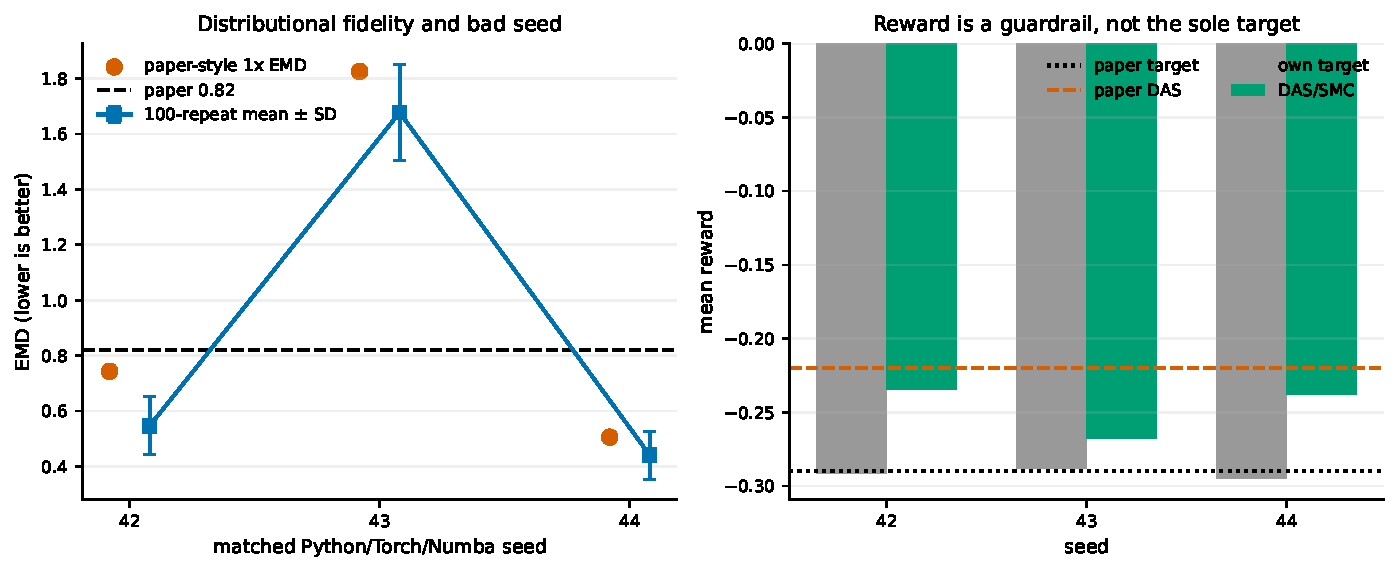
\includegraphics[width=.94\textwidth,height=.70\textheight,keepaspectratio]{assets/fig_das_rescue_variance.pdf}
  \vspace{-.06cm}
  \small
  \good{seed 42: 9.8\% from paper}\quad $1.025\pm0.704$ across seeds \quad \warn{worst: 1.826}
  \papersource{Reproduction figure from results/das\_rescue\_multiseed.json}
\end{frame}

% 6 DAS 4/5
\begin{frame}{All DAS seeds cover 3/3 modes, yet mass allocation still differs}
  \centering
  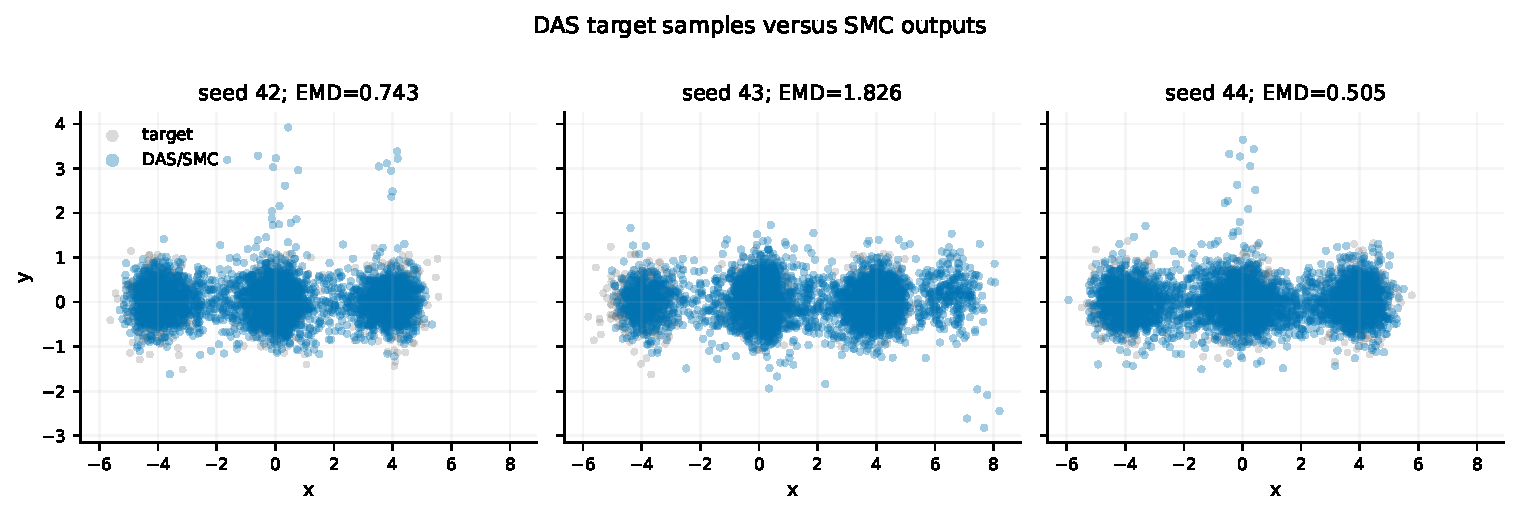
\includegraphics[width=.96\textwidth,height=.72\textheight,keepaspectratio]{assets/fig_das_rescue_samples.pdf}
  \vspace{-.08cm}
  \small
  Seed 43: \good{3/3 modes}\quad \warn{mass $L_1=0.420$}\quad \warn{EMD $=1.826$}
  \papersource{Saved target/SMC arrays; results/das\_rescue\_multiseed.json}
\end{frame}

% 7 DAS 5/5
\begin{frame}{Kaggle T4x2 executes the payload, but does not reproduce the number}
  \centering
  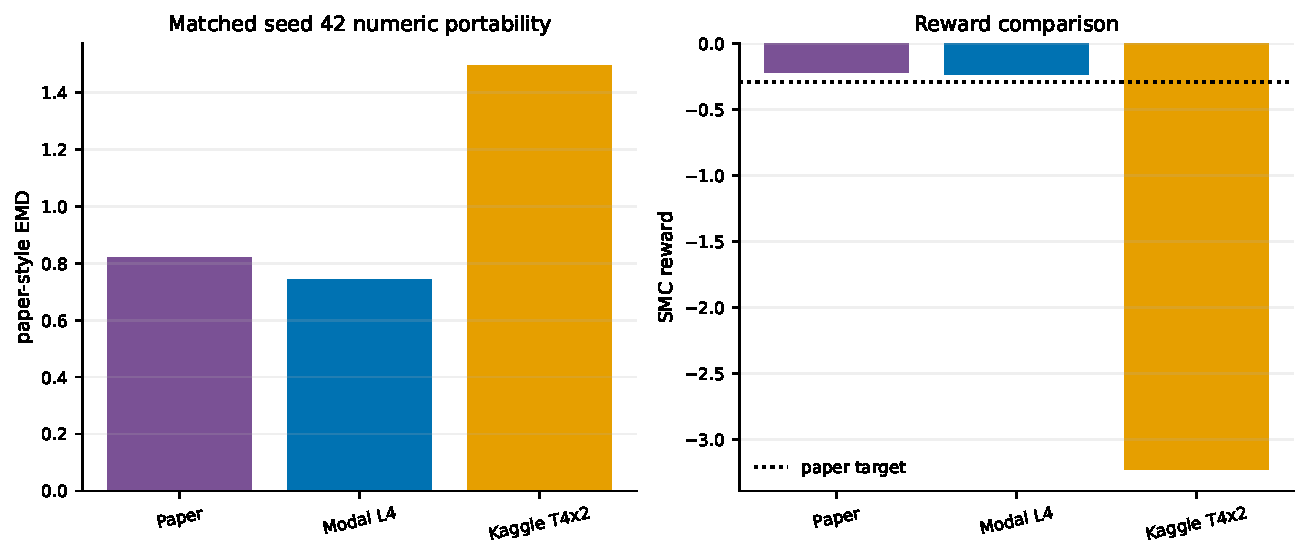
\includegraphics[width=.88\textwidth,height=.66\textheight,keepaspectratio]{assets/fig_das_kaggle_rescue.pdf}
  \vspace{-.06cm}
  \small
  \good{Infrastructure pass: 2 Tesla T4 visible}\quad
  \bad{Paper match fail: EMD 1.496 vs 0.820}\quad
  \bad{Modal portability fail: 67.2\% symmetric difference}

  \scriptsize T4x2 = allocation/portability test; upstream workload uses one GPU.
  \papersource{Kaggle r6 artifact; results/das\_kaggle\_t4x2\_rescue.json}
\end{frame}

% 8 FK Steering 1/4
\begin{frame}{FK Steering: a general particle framework, reproduced at one prompt}
  \normalsize
  \begin{columns}[T,onlytextwidth]
    \begin{column}{.54\textwidth}
      \metricbox{Configuration}{%
        ``brown knife + blue donut''\\
        SD 2.1 mirror · seeds 42--44\\
        $k=4$ · 100 steps · $\lambda=2$}
      \vspace{.28cm}
      \metricbox{Potential rules}{%
        FK-max: best reward so far\\
        FK-difference: reward increment\\
        ESS $\rightarrow$ resample}
    \end{column}
    \begin{column}{.42\textwidth}
      \begin{beamercolorbox}[rounded=true,sep=.7em,wd=\linewidth]{block body}
        \centering
        $x_t^{1:k}$\\[-2pt]
        $\downarrow$ proposal\\[-2pt]
        reward potential $G_t$\\[-2pt]
        $\downarrow$ weight / ESS / resample\\[-2pt]
        $x_{t-1}^{1:k}$
      \end{beamercolorbox}
      \vspace{.30cm}
      \warn{Identity caveat}\par\smallskip
      Upstream checkpoint: 401\\
      Run: public mirror
    \end{column}
  \end{columns}
  \papersource{FK Steering paper; upstream commit 9413005; results/fk\_steering\_one\_prompt.json}
\end{frame}

% 9 FK Steering 2/4
\begin{frame}{FK Steering metric: average ImageReward across all four particles}
  \normalsize
  \begin{columns}[T,onlytextwidth]
    \begin{column}{.55\textwidth}
      \metricbox{Per method and seed}{%
        \[\bar R_{m,s}=\frac{1}{4}\sum_{j=1}^{4}S_{\mathrm{IR}}(x_{m,s,j},c).\]
        \centering learned image--text score · higher is better}
      \vspace{.25cm}
      \metricbox{Aggregation}{mean $\pm$ sample SD across three seeds\\
      all particles retained}
    \end{column}
    \begin{column}{.41\textwidth}
      \centering
      \begin{tabular}{@{}lrr@{}}
        \toprule
        Method & mean & SD \\
        \midrule
        FK-max & 0.429 & 0.625 \\
        FK-difference & 1.161 & 0.938 \\
        Base & 0.660 & 0.541 \\
        \bottomrule
      \end{tabular}
      \vspace{.34cm}
      \warn{Best-of-4 $\neq$ population mean}
    \end{column}
  \end{columns}
  \papersource{ImageReward aggregation reconstructed from the saved nine generations and final\_metrics.json}
\end{frame}

% 10 FK Steering 3/4
\begin{frame}{FK Steering: ranking flips across three seeds}
  \centering
  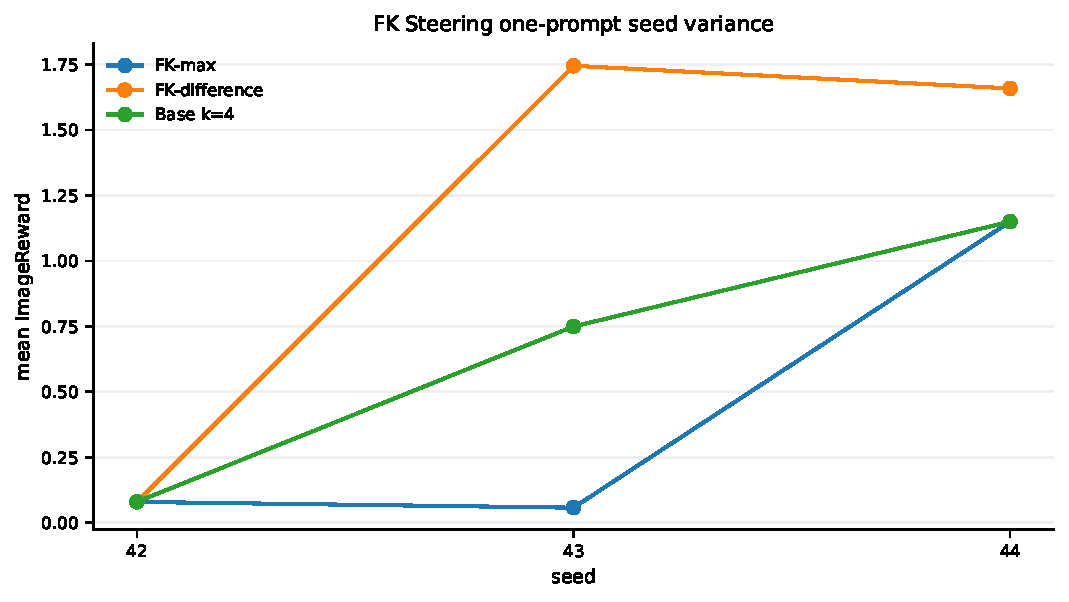
\includegraphics[width=.86\textwidth,height=.68\textheight,keepaspectratio]{assets/fig_fk_steering_variance_final.pdf}
  \vspace{-.08cm}
  \small
  \begin{tabular}{ccc}
    \warn{ranking flips} & seed 42: all equal & seed 44: FK-max = base
  \end{tabular}
  \papersource{Reproduction figure from results/fk\_steering\_one\_prompt.json}
\end{frame}

% 11 FK Steering 4/4
\begin{frame}{FK Steering produces plausible samples; the scientific claim remains partial}
  \centering
  \begin{columns}[T,onlytextwidth]
    \begin{column}{.32\textwidth}
      \centering\scriptsize FK-max, seed 43\\[2pt]
      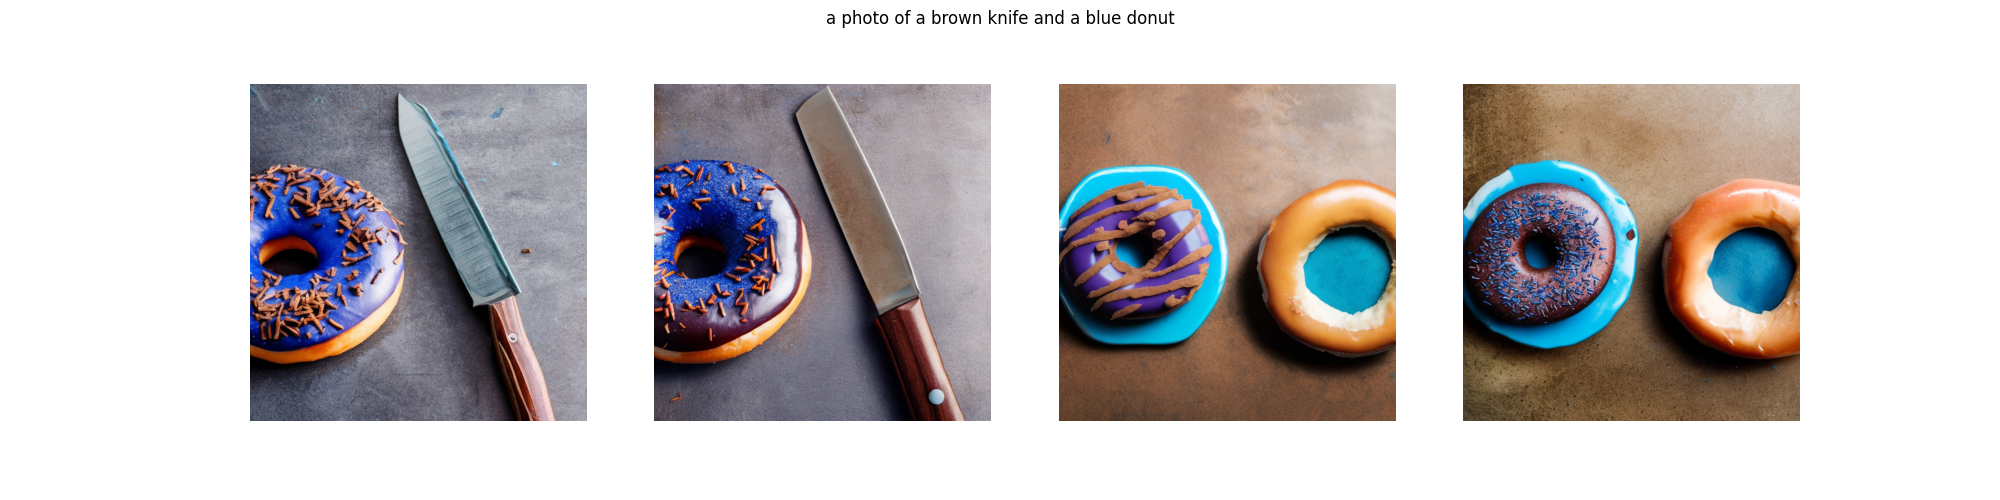
\includegraphics[width=\linewidth]{assets/fk_seed43_max.png}
    \end{column}
    \begin{column}{.32\textwidth}
      \centering\scriptsize FK-difference, seed 43\\[2pt]
      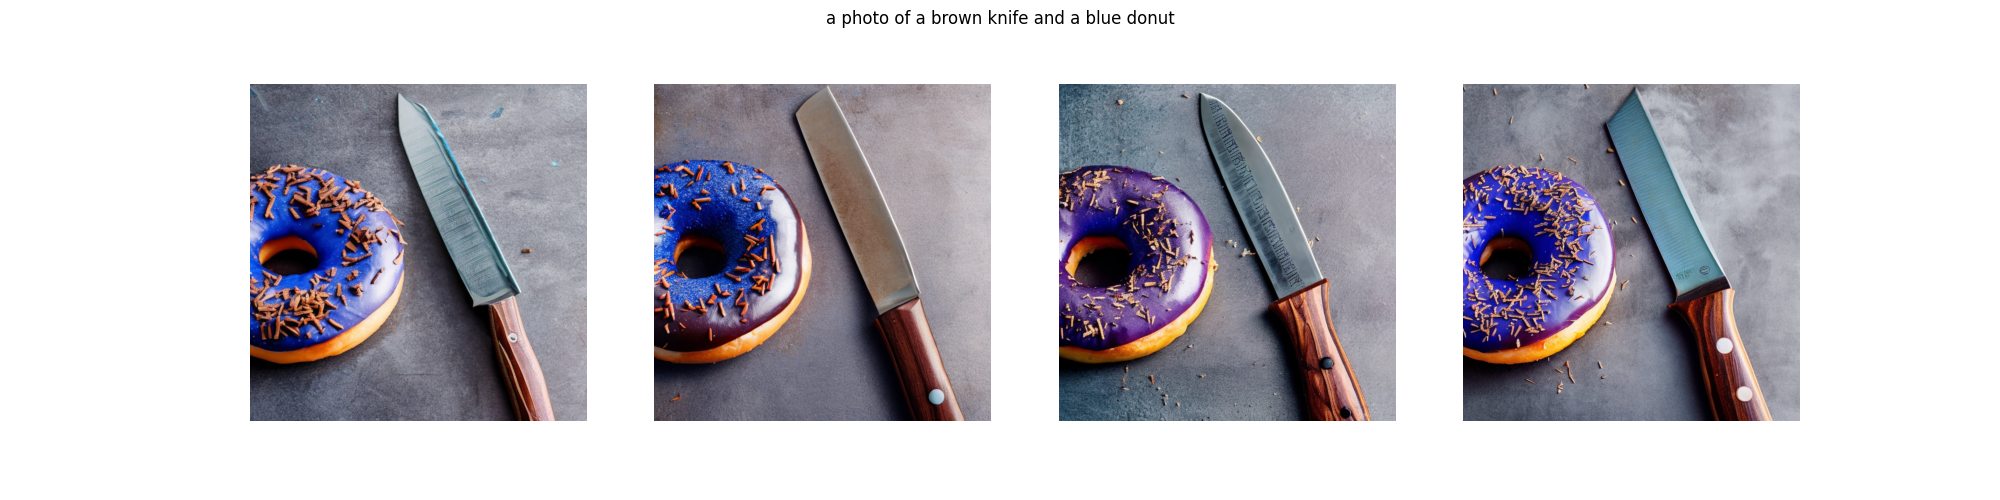
\includegraphics[width=\linewidth]{assets/fk_seed43_diff.png}
    \end{column}
    \begin{column}{.32\textwidth}
      \centering\scriptsize Base, seed 43\\[2pt]
      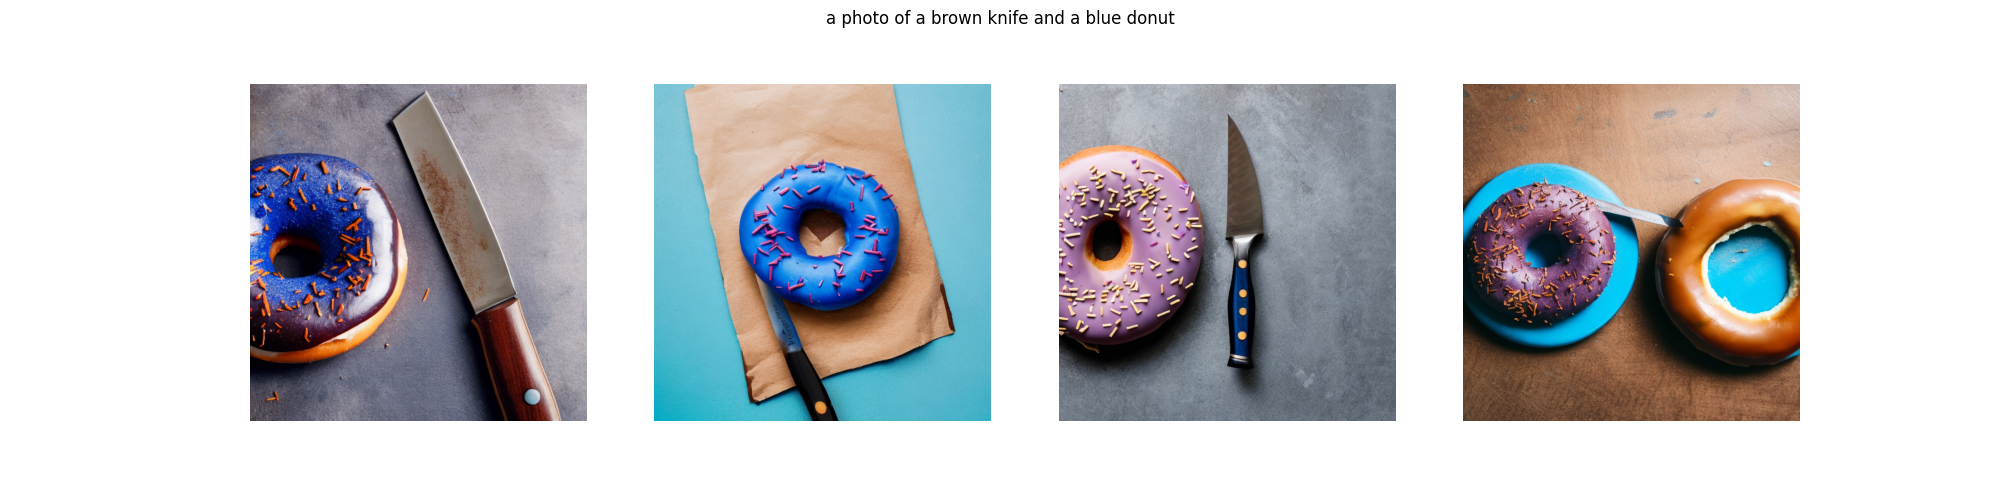
\includegraphics[width=\linewidth]{assets/fk_seed43_base.png}
    \end{column}
  \end{columns}
  \vspace{.32cm}
  \begin{beamercolorbox}[rounded=true,sep=.55em,wd=.92\linewidth]{block body}
    \small\centering
    \good{Scientific payload complete}\quad
    \warn{one prompt + three seeds}\quad
    \bad{not a GenEval reproduction or superiority claim}
  \end{beamercolorbox}
  \papersource{Saved remote grids; one-prompt evidence only}
\end{frame}

% 12 FKC 1/5
\begin{frame}{FK Correctors: exact Table A1 protocol}
  \normalsize
  \begin{columns}[T,onlytextwidth]
    \begin{column}{.56\textwidth}
      \centering
      \begin{tabular}{@{}lr@{}}
        \toprule
        Protocol item & Reproduction \\
        \midrule
        Samples per run & 10,000 \\
        Integration steps & 1,000 \\
        Step size $dt$ & 0.001 \\
        Stochastic runs & 5 \\
        Proposals & target score, tempered noise \\
        Correctors & none, BDC, systematic \\
        Metric cells & $6\times5=30$ \\
        \bottomrule
      \end{tabular}
    \end{column}
    \begin{column}{.40\textwidth}
      \metricbox{Runtime repair}{Forward one existing BDC shape flag.\\[3pt]
      Hashes retained · upstream clean.}
      \vspace{.28cm}
      \good{17.4 min}\;\good{7.99 GiB}\;\good{\$0.367}
    \end{column}
  \end{columns}
  \papersource{FK Correctors Table A1; upstream commit aa6f5ed; exact-run manifest}
\end{frame}

% 13 FKC 2/5
\begin{frame}{FK Correctors metrics compare different projections of error}
  \normalsize
  \begin{columns}[T,onlytextwidth]
    \begin{column}{.48\textwidth}
      \metricbox{$W_1$ and $W_2$ $\downarrow$}{%
        \[W_p=\left[\min_{\pi}\sum_{ij}\pi_{ij}\|x_i-y_j\|_2^p\right]^{1/p}.\]
        2D transport · $W_2$ penalizes long moves.}
      \vspace{.20cm}
      \metricbox{MMD $\downarrow$}{biased $\widehat{\mathrm{MMD}}^2$ · 10 RBF kernels\\
      bandwidth-dependent scale}
    \end{column}
    \begin{column}{.48\textwidth}
      \metricbox{TV $\downarrow$}{$200\times200$ histogram\\
        $\widehat{\mathrm{TV}}=\frac12\sum_b|\hat p_b-\hat q_b|$\\
        grid/bin-dependent}
      \vspace{.20cm}
      \metricbox{Energy-W2 $\downarrow$}{$x\mapsto E(x)$ · 1D transport\\
      implementation returns $W_2^2$, not $W_2$}
    \end{column}
  \end{columns}
  \papersource{Metric definitions audited against the official FK Correctors notebook}
\end{frame}

% 14 FKC 3/5
\begin{frame}{Energy-W2 is squared transport between energy histograms}
  \normalsize
  \begin{columns}[T,onlytextwidth]
    \begin{column}{.54\textwidth}
      \metricbox{Code semantics}{%
        \texttt{pot.emd2\_1d} · squared cost · no square root
        \[\begin{aligned}
        D_E&=\min_{\gamma}\sum_{ij}\gamma_{ij}|E(x_i)-E(y_j)|^2\\
           &=W_2^2(E_\#X,E_\#Y).
        \end{aligned}\]
        $E_\#X$: distribution of scalar energy only.}
      \vspace{.24cm}
      \begin{itemize}
        \item Units: energy$^2$; $E\mapsto2E \Rightarrow D_E\mapsto4D_E$.
        \item Not a measure of 2D sample geometry.
      \end{itemize}
    \end{column}
    \begin{column}{.42\textwidth}
      \metricbox{$D_E=0$, but geometry differs}{%
        $E(x)=\|x\|_2^2$,\\
        $X=\{(-1,0),(1,0)\}$,\\
        $Y=\{(0,-1),(0,1)\}$.\\[3pt]
        $E_\#X=E_\#Y=\delta_1 \Rightarrow D_E=0$,\\[5pt]
        $W_1(X,Y)=W_2(X,Y)=\sqrt2>0$.}
    \end{column}
  \end{columns}
  \papersource{Implementation semantics: official notebook call to pot.emd2\_1d; example is explanatory}
\end{frame}

% 15 FKC 4/5
\begin{frame}{FK Correctors reproduces all 30 Table A1 cells within $\pm2$ paper SD}
  \centering
  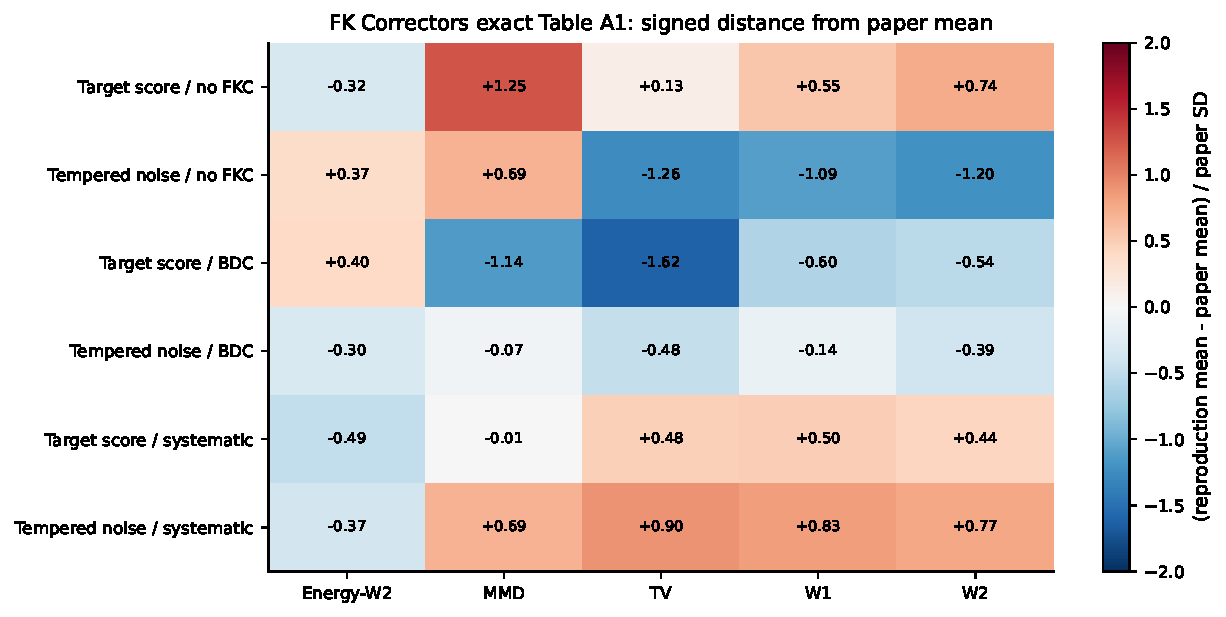
\includegraphics[width=.84\textwidth,height=.68\textheight,keepaspectratio]{assets/fig_fkc_relative_error_final.pdf}
  \vspace{-.08cm}
  \small
  \good{30/30 within $\pm2$ SD}\quad\good{24/30 within $\pm1$ SD}\quad\warn{19/20 correction directions agree}

  \scriptsize $\pm$SD is a compatibility band, not an equivalence test.
  \papersource{Exact Table A1 aggregation: results/fk\_correctors\_table\_a1\_exact.json}
\end{frame}

% 16 FKC 5/5
\begin{frame}{FK Correctors: compatible means hide bad runs}
  \centering
  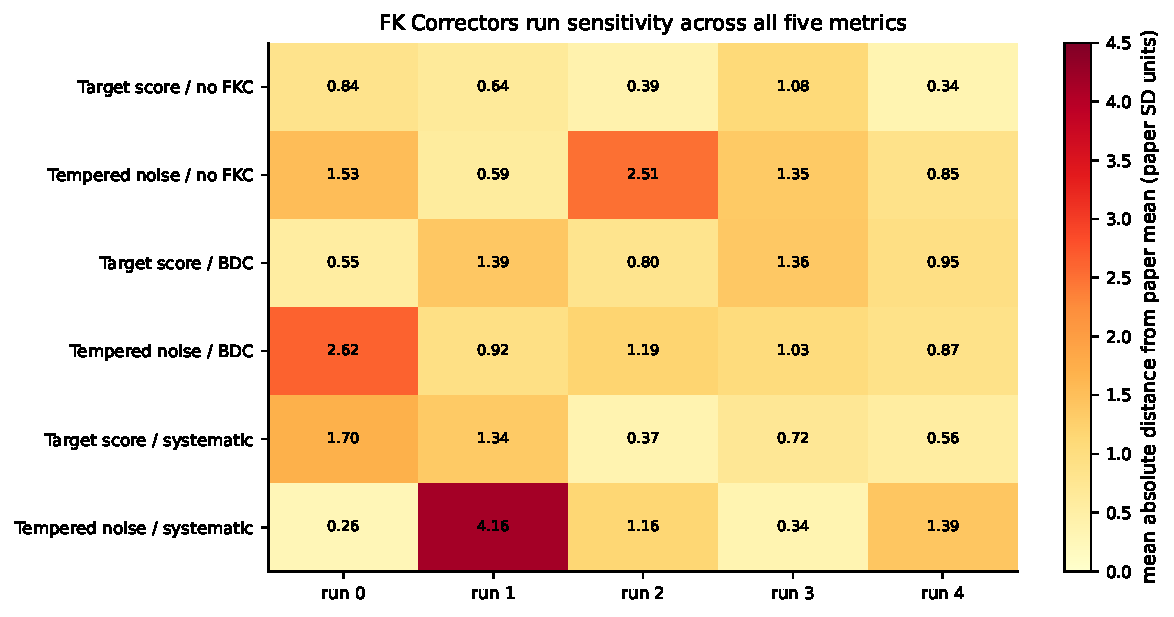
\includegraphics[width=.84\textwidth,height=.67\textheight,keepaspectratio]{assets/fig_fkc_run_variance_final.pdf}
  \vspace{-.08cm}
  \small
  \begin{tabular}{cc}
    BDC run 0: $W_2=29.925$ & systematic run 1: $W_2=20.849$
  \end{tabular}

  \centering\warn{Verdict: PASS WITH VARIANCE -- exact protocol and means match, run stability does not.}
  \papersource{Five sequential stochastic runs; upstream loop does not explicitly reseed}
\end{frame}

% 17 Null-TTA 1/5
\begin{frame}{Null-TTA: optimize only the null-text embedding at inference}
  \normalsize
  \begin{columns}[T,onlytextwidth]
    \begin{column}{.55\textwidth}
      \metricbox{Target}{Table 1 · SD-v1.5 · PickScore\\
      $n_{\max}=55$ · diffusion weights frozen}
      \vspace{.24cm}
      \begin{itemize}
        \item 50 prompts $\times$ 3 seeds $=150$ pairs.
        \item $K=3$ · 100 steps · $n:5\rightarrow55$.
        \item Same prompt/seed: baseline vs optimized.
      \end{itemize}
    \end{column}
    \begin{column}{.41\textwidth}
      \metricbox{PickScore $\uparrow$}{cosine(normalized image, text)\\
      no softmax · not a probability}
      \vspace{.24cm}
      \metricbox{Gate}{symmetric difference $\leq10\%$\\
      95\% CI$(\Delta)$ entirely $>0$}
    \end{column}
  \end{columns}
  \papersource{Null-TTA official code commit 337bf73; results/null\_tta\_table1.json}
\end{frame}

% 18 Null-TTA 2/5
\begin{frame}{Null-TTA: three secondary alignment proxies}
  \normalsize
  \begin{columns}[T,onlytextwidth]
    \begin{column}{.32\textwidth}
      \metricbox{HPS v2 $\uparrow$}{held-out text--image preference proxy}
    \end{column}
    \begin{column}{.32\textwidth}
      \metricbox{Aesthetic $\uparrow$}{image-only CLIP feature $\rightarrow$ MLP}
    \end{column}
    \begin{column}{.32\textwidth}
      \metricbox{ImageReward $\uparrow$}{BLIP image--text reward · unbounded}
    \end{column}
  \end{columns}
  \vspace{.22cm}
  \begin{beamercolorbox}[rounded=true,sep=.65em,wd=.92\linewidth]{block body}
    \centering
    Proxy agreement supports transfer; \textbf{none replaces human evaluation}.
  \end{beamercolorbox}
  \papersource{Scorer implementations and checkpoints audited in the reproduction report}
\end{frame}

% 19 Null-TTA 3/5
\begin{frame}{Null-TTA matches all four Table 1 point estimates}
  \centering
  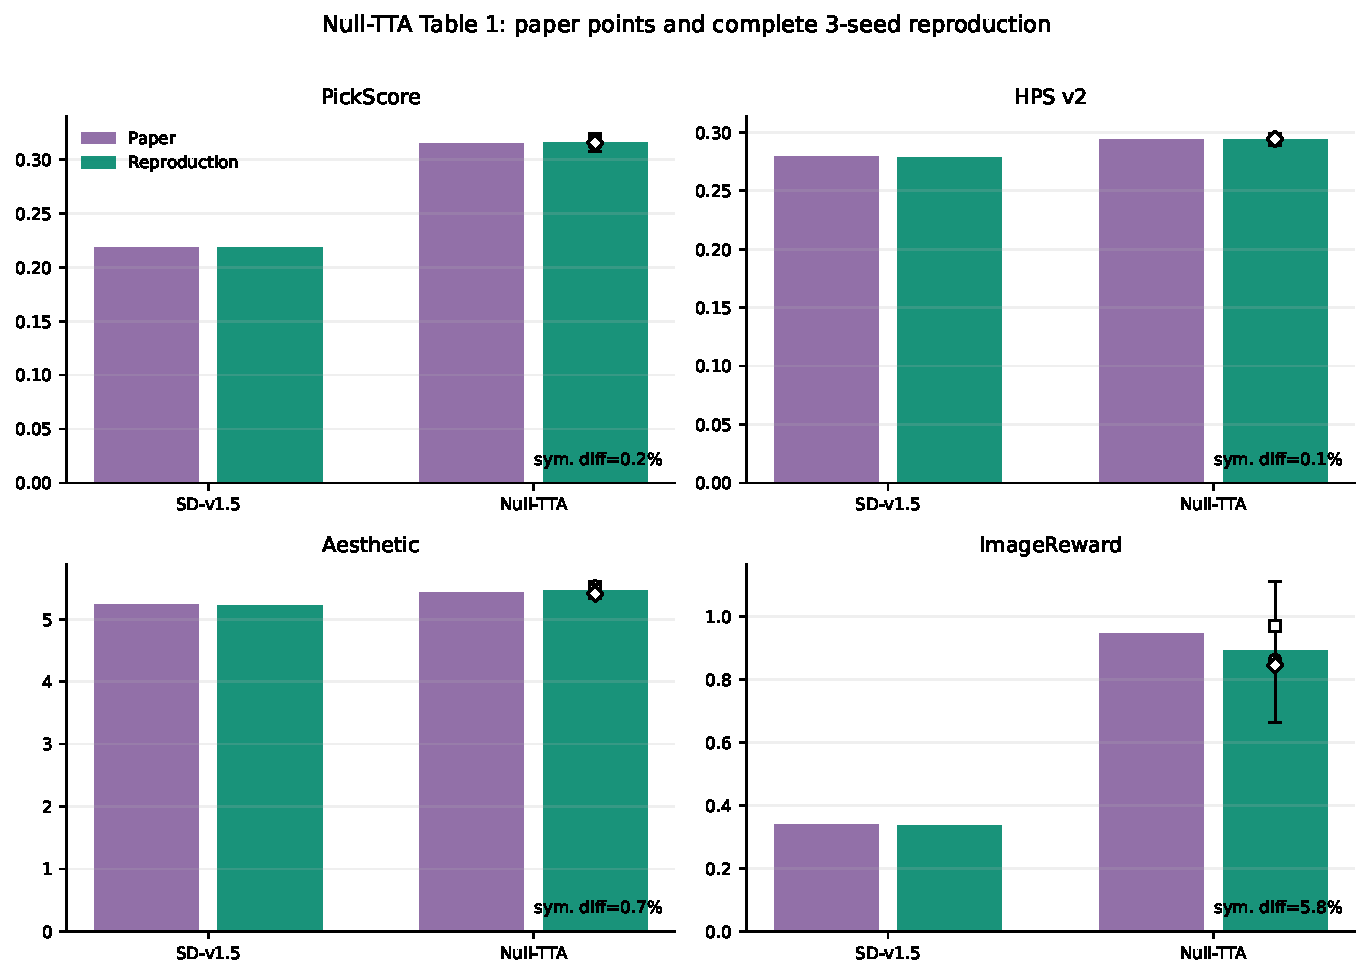
\includegraphics[width=.88\textwidth,height=.68\textheight,keepaspectratio]{assets/fig_null_tta_table1.pdf}
  \vspace{-.08cm}
  \small
  \begin{tabular}{cccc}
    PickScore & HPS v2 & Aesthetic & ImageReward \\
    \good{0.2\%} & \good{0.1\%} & \good{0.7\%} & \good{5.8\%}
  \end{tabular}
  \papersource{Paper and reproduction rows from results/null\_tta\_table1.json}
\end{frame}

% 20 Null-TTA 4/5
\begin{frame}{Null-TTA: stable PickScore gain across seeds}
  \centering
  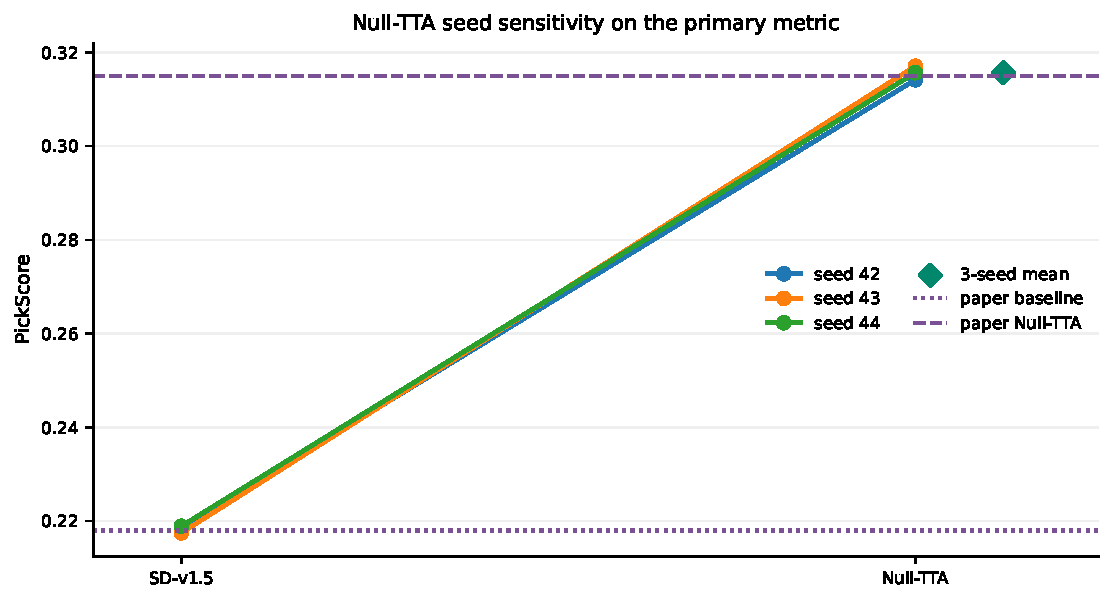
\includegraphics[width=.88\textwidth,height=.67\textheight,keepaspectratio]{assets/fig_null_tta_seed_variance.pdf}
  \vspace{-.08cm}
  \small
  \begin{tabular}{cccc}
    repro & paper & paired gain & 95\% CI \\
    \good{0.316} & $0.315$ & $0.097$ & \good{$[0.089,0.106]$}
  \end{tabular}
  \papersource{50 prompts per seed; hierarchical bootstrap resamples seed then prompt, 10,000 repeats}
\end{frame}

% 21 Null-TTA 5/5
\begin{frame}{Null-TTA: qualitative pairs support the scoped result}
  \centering
  \begin{columns}[T,onlytextwidth]
    \begin{column}{.24\textwidth}
      \centering\scriptsize Bus: baseline, PickScore 0.213\\[2pt]
      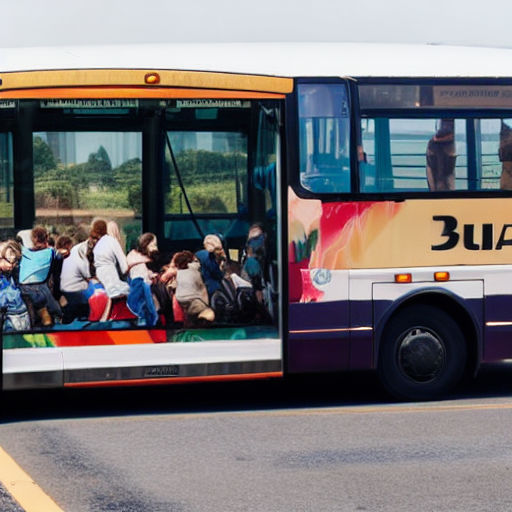
\includegraphics[width=.88\linewidth]{assets/null_bus_base.png}
    \end{column}
    \begin{column}{.24\textwidth}
      \centering\scriptsize Bus: optimized, 0.313\\[2pt]
      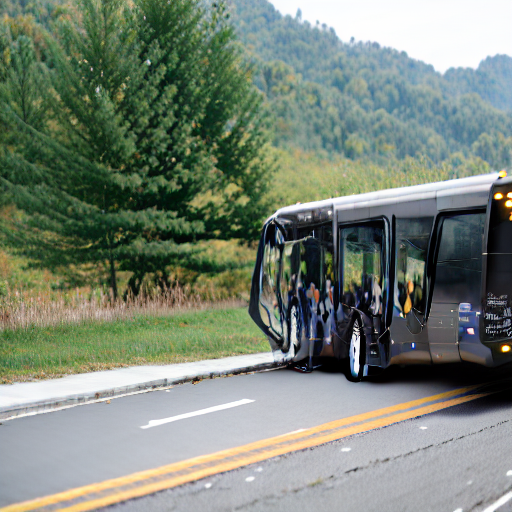
\includegraphics[width=.88\linewidth]{assets/null_bus_opt.png}
    \end{column}
    \begin{column}{.24\textwidth}
      \centering\scriptsize Bikes: baseline, 0.226\\[2pt]
      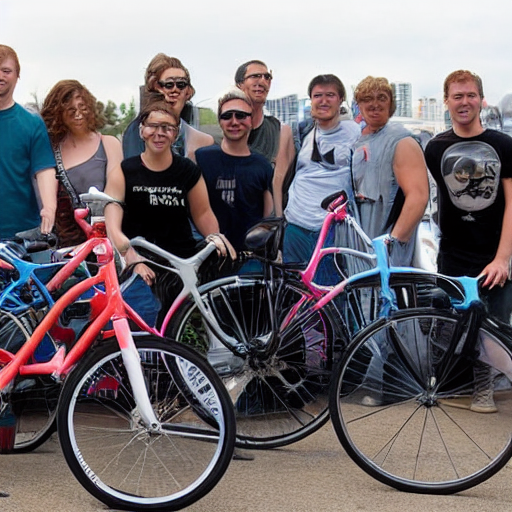
\includegraphics[width=.88\linewidth]{assets/null_bikes_base.png}
    \end{column}
    \begin{column}{.24\textwidth}
      \centering\scriptsize Bikes: optimized, 0.330\\[2pt]
      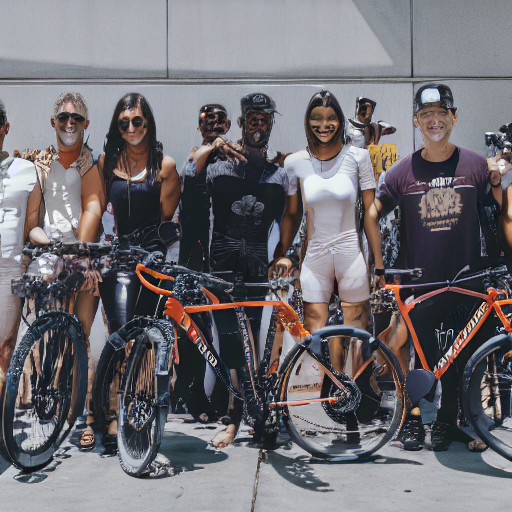
\includegraphics[width=.88\linewidth]{assets/null_bikes_opt.png}
    \end{column}
  \end{columns}
  \vspace{.32cm}
  \begin{beamercolorbox}[rounded=true,sep=.55em,wd=.92\linewidth]{block body}
    \small\centering
    \good{PASS for SD-v1.5 Table 1}\quad
    \warn{not evidence for SDXL, other rewards, or universal human preference}
  \end{beamercolorbox}
  \papersource{Seed 44 official PNG artifacts; prompts 0--1; PickScore from saved CSV}
\end{frame}

% 22
\begin{frame}{What the reproduction supports -- and what it does not}
  \normalsize
  \renewcommand{\arraystretch}{1.25}
  \begin{tabular}{@{}>{\raggedright\arraybackslash}p{2.5cm}>{\raggedright\arraybackslash}p{3.0cm}>{\raggedright\arraybackslash}p{6.9cm}@{}}
    \toprule
    Paper & Verdict & Evidence boundary \\
    \midrule
    DAS & \warn{PASS + VAR} & seed 42 matches · seed variance · Kaggle fail \\
    FK Steering & \warn{PARTIAL} & one prompt · three seeds · model mirror \\
    FK Correctors & \warn{PASS + VAR} & 30/30 compatible · bad sequential runs \\
    Null-TTA & \good{PASS} & 150 pairs · four metrics · SD-v1.5 only \\
    \bottomrule
  \end{tabular}
  \vspace{.18cm}
  \begin{beamercolorbox}[rounded=true,sep=.75em,wd=.94\linewidth]{block body}
    \centering\large
    Narrow · stable · traceable claims beat the best-looking score.
  \end{beamercolorbox}
  \papersource{All verdicts are scoped to executed artifacts; no benchmark-wide extrapolation}
\end{frame}

\end{document}
